\documentclass{article}

\usepackage[utf8]{inputenc}
\usepackage{amsmath}
\usepackage{amsfonts}
\usepackage{amssymb}
\usepackage{graphicx}
\usepackage[table,xcdraw]{xcolor}
\usepackage[hidelinks]{hyperref}
\usepackage{fontawesome5}


\graphicspath{ {./images/} }

\renewcommand{\contentsname}{Indice}

\makeatletter
\newcommand*{\rom}[1]{\expandafter\@slowromancap\romannumeral #1@}
\makeatother

\usepackage[a4paper,top=2cm,bottom=2cm,left=2cm,right=2cm]{geometry}


\title{\textbf{\Huge Analisi dei Requisiti}}
\author{Edoardo Ghirardello, Giulio Cappelli, Elia Casotti \\ \\ Gruppo T42}
\date{2022}

\let\origthesubsubsection\thesubsubsection

\begin{document}

\maketitle

\clearpage
\tableofcontents
\clearpage

\section{Scopo del documento}
\begin{description}
    \item[] In questo documento si riporta la descrizione e il funzionamento dell'applicazione "Fen Festa" in linguaggio naturale.
    \item[] Verranno analizzati gli obiettivi del progetto, definiti i requisiti funzionali e non funzionali e infine verranno esposti i requisiti di front-end e di back-end.
\end{description}
\clearpage
\section{Obiettivi del progetto}
\begin{description}
    \item[] Data la difficoltà nella ricerca di attività serali con cui potersi svagare a Trento, siamo giunti alla conclusione che sarebbe utile un’applicazione raggruppante tutti gli eventi disponibili nelle varie serate, presenti in città e dintorni.
    \item[] L’applicazione, chiamata “Fen Festa”:
          \begin{itemize}
              \item aiuta gli utenti base a trovare la proposta che fa per loro, facendo visualizzare un calendario nel quale sono segnati tutti gli eventi disponibili in quella serata (o nelle successive), coadiuvati da un’immagine, un titolo, posizione e una descrizione dell’evento
              \item l’utente può, oltre che salvare nei preferiti l’evento, comunicare la sua partecipazione
              \item permette agli organizzatori di eventi, gestori di bar e simili, di inserire le loro proposte nell’applicazione, tramite un form precompilato
              \item permette di salvarsi gli eventi a cui l’utente è interessato e a poter ricevere una notifica nella giornata in cui sono stati programmati
          \end{itemize}
\end{description}
\clearpage
\section{Requisiti}
\begin{description}
    \item[] Vengono definiti 4 tipi di utente:
          \begin{itemize}
              \item Utente non registrato (\textbf{UNR})
              \item Utente registrato (\textbf{UR})
              \item Utente organizzatore (\textbf{UO})
              \item Utente admin (\textbf{UA})
          \end{itemize}
\end{description}
\subsection{Requisiti Funzionali (RF)}
\renewcommand\thesubsubsection{RF\arabic{subsubsection}}
\subsubsection{Visualizzazione eventi} \label{rf_1}
\begin{description}
    \item[] Si applica a: \textbf{UNR}, \textbf{UR}, \textbf{UO}, \textbf{UA}
    \item[] L'utente può visualizzare l'elenco degli eventi attraverso un calendario (Giornaliero, Settimanale, Mensile) o può visualizzare una mappa indicante gli eventi del giorno con la loro posizione
\end{description}
\subsubsection{Ricerca Eventi} \label{rf_2}
\begin{description}
    \item[] Si applica a: \textbf{UNR}, \textbf{UR}, \textbf{UO}, \textbf{UA}
    \item[] L'utente può ricercare un evento specifico tramite keyword o tag ottenendo in risposta una lista di risultati inerenti
\end{description}
\subsubsection{Visualizzazione descrizione evento (Utente Non Registrato)} \label{rf_3}
\begin{description}
    \item[] Si applica a: \textbf{UNR}
    \item[] L'utente non registrato una volta selezionato l'evento dal calendario visualizza i dettagli dell'evento, visualizzando:
          \begin{itemize}
              \item Nome
              \item Immagine
              \item Descrizione
              \item Tag
              \item Data e Ora
              \item Luogo (Posizione/Indirizzo)
              \item Numero partecipanti
          \end{itemize}
\end{description}
\subsubsection{Visualizzazione descrizione evento (Utente Registrato)} \label{rf_4}
\begin{description}
    \item[] Si applica a: \textbf{UR}, \textbf{UO}, \textbf{UA}
    \item[] L'utente registrato una volta selezionato l'evento dal calendario visualizza i dettagli dell'evento, quali:
          \begin{itemize}
              \item Nome
              \item Immagine
              \item Descrizione
              \item Tag
              \item Data e Ora
              \item Luogo (Posizione/Indirizzo)
              \item Numero partecipanti
              \item Tasto "Partecipo"
              \item Tasto "Salva Evento"
          \end{itemize}
\end{description}
\subsubsection{Creazione evento} \label{rf_5}
\begin{description}
    \item[] Si applica a: \textbf{UO}, \textbf{UA}
    \item[] L'utente organizzatore o admin possono creare un nuovo evento compilando l'apposito form:
          \begin{itemize}
              \item Nome
              \item Immagine
              \item Descrizione
              \item Tag
              \item Data e Ora
              \item Luogo (Posizione/Indirizzo)
          \end{itemize}
\end{description}
\subsubsection{Modifica evento} \label{rf_6}
\begin{description}
    \item[] Si applica a: \textbf{UO}, \textbf{UA}
    \item[] L'utente organizzatore o admin possono modificare un evento attraverso l'apposito form:
          \begin{itemize}
              \item Nome
              \item Immagine
              \item Descrizione
              \item Tag
              \item Data e Ora
              \item Luogo (Posizione/Indirizzo)
          \end{itemize}
\end{description}
\subsubsection{Eliminazione evento} \label{rf_7}
\begin{description}
    \item[] Si applica a: \textbf{UO}, \textbf{UA}
    \item[] L'utente organizzatore o admin possono eliminare un evento
\end{description}
\subsubsection{Login} \label{rf_8}
\begin{description}
    \item[] Si applica a: \textbf{UNR}
    \item[] L'utente non registrato se ha già un account può effettuare il login inserendo:
          \begin{itemize}
              \item Email
              \item Password
          \end{itemize}
\end{description}
\subsubsection{Recupero password} \label{rf_9}
\begin{description}
    \item[] Si applica a: \textbf{UNR}
    \item[] L'utente non registrato se si è dimenticato la password può richiedere di resettarla così ne può impostarne un'altra
\end{description}
\subsubsection{Creazione account utente} \label{rf_10}
\begin{description}
    \item[] Si applica a: \textbf{UNR}
    \item[] L'utente non registrato può registrarsi tramite apposito form inserendo
          \begin{itemize}
              \item Email
              \item Password
              \item Conferma della Password
          \end{itemize}
\end{description}
\subsubsection{Conferma creazione account} \label{}
\begin{description}
    \item[] Si applica a: \textbf{UNR}
    \item[] L'utente non registrato una volta creato l'account deve confermarlo attraverso un link inviato via mail
\end{description}
\subsubsection{Modifica profilo utente} \label{rf_10}
\begin{description}
    \item[] Si applica a: \textbf{UR}
    \item[] L'utente registrato può cambiare la propria password ed eliminare il proprio profilo
\end{description}
\subsubsection{Modifica profilo utente organizzatore} \label{rf_11}
\begin{description}
    \item[] Si applica a: \textbf{UO}
    \item[] L'utente organizzatore può scegliere un alias con cui farsi riconoscere e può inserire un immagine di profilo
    \item[] L'utente organizzatore può cambiare la propria password ed eliminare il proprio profilo
\end{description}
\subsubsection{Richiesta upgrade a utente organizzatore} \label{rf_12}
\begin{description}
    \item[] Si applica a: \textbf{UR}
    \item[] L'utente registrato può, dalla pagina del proprio profilo, fare richiesta di upgrade a utente organizzatore. Dopo aver compilato apposito form (nome organizzazione e tipologia di eventi di cui si occupa) verrà inviata una richiesta all'amministratore (mail)
\end{description}
\subsubsection{Consegna e Revoca Privilegi} \label{rf_13}
\begin{description}
    \item[] Si applica a: \textbf{UA}
    \item[] L'utente admin può cambiare i permessi degli altri utenti, rendendoli \textbf{UO} oppure declassarli a \textbf{UR}
\end{description}
\clearpage
\renewcommand\thesubsubsection{\origthesubsubsection}
\subsection{Requisiti Non Funzionali (RNF)}
\renewcommand\thesubsubsection{RNF\arabic{subsubsection}}
\subsubsection{Privacy} \label{rnf_1}
\begin{description}
    \item[] L’applicazione deve essere progettata e realizzata in ottemperanza alle vigenti disposizioni di legge in materia di tutela della privacy e trattamento dei dati, nello specifico anche al Regolamento Europeo per la protezione dei dati (GDPR).
    \item[] L’applicazione non permetterà ai suoi operatori di conoscere alcuna informazione personale (a esclusione del DPO) sui clienti, eccetto la mail
\end{description}
\subsubsection{Sicurezza} \label{rnf_2}
\begin{description}
    \item[] L’applicazione deve garantire la riservatezza delle informazioni.
    \item[] È necessario assicurarsi che ogni utente veda e possa vedere solamente i propri dati.
\end{description}
\subsubsection{Scalabilità} \label{rnf_3}
\begin{description}
    \item[] L'applicazione deve garantire l'accesso simultaneo di un numero crescente e variabile di utenti
    \item[] Deve garantire l'accesso simultaneo ad almeno 100 utenti
\end{description}
\subsubsection{Affidabilità} \label{rnf_4}
\begin{description}
    \item[] Il sistema si occupa di eseguire backup periodici per evitare perdite dei dati degli utenti
\end{description}
\subsubsection{Memorizzazione} \label{rnf_5}
\begin{description}
    \item[] I dati utente e i vari eventi vengono salvati su database senza quindi occupare più memoria del necessario all'utente
\end{description}
\subsubsection{Compatibilità e Accessibilità} \label{rnf_6}
\begin{description}
    \item[] L’applicazione deve essere compatibile con Android 8.0 / iOS 12 e successivi e i principali Browser web (Chrome, Safari, Edge, \dots)
\end{description}
\subsubsection{Supportabilità} \label{rnf_7}
\begin{description}
    \item[] L'app è facilmente utilizzabile tramite web
\end{description}
\subsubsection{Facilità di utilizzo} \label{rnf_8}
\begin{description}
    \item[] Il sistema permette d'ingrandire la mappa visualizzando meglio la locazione dell'evento
    \item[] Il sistema permette di cambiare tra dark mode e light mode
    \item[] Il sistema permette di spostarsi tra le varie schermate in modo intuitivo
\end{description}
\renewcommand\thesubsubsection{\origthesubsubsection}
\clearpage
\section{Front-End}
\begin{description}
    \item[] L'applicazione sarà composta da un sito disponibile sia per smartphone, che per pc
    \item[] In questa sezione vengono riportati alcuni mock-up del front-end per smartphone
          \begin{enumerate}
              \item Pagina home con calendario
              \item Pagina home con mappa
              \item Pagina creazione evento
          \end{enumerate}
\end{description}
\subsection{Pagina home con calendario}
\begin{description}
    \item[] Utenti utilizzatori: \textbf{UNR}, \textbf{UR}, \textbf{UO}, \textbf{UA}
    \item[] Requisiti interessati: \hyperref[rf_1]{\textbf{RF1}}, \hyperref[rf_2]{\textbf{RF2}}
    \item[] \begin{center}
              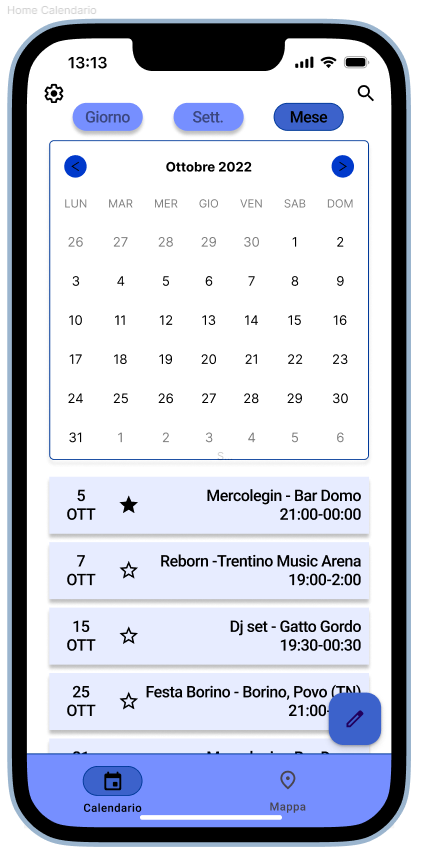
\includegraphics[scale=0.6]{Home_Calendario.png}
          \end{center}
    \item[] In questa schermata si possono visualizzare gli eventi giornalieri, settimanali o mensili.
    \item[] Selezionando un giorno nel calendario compariranno nell'elenco solo gli eventi relativi a quella giornata.
    \item[] Cliccando su un evento se ne potranno visualizzare i dettagli
    \item[] Premendo l'icona "\faIcon{search}" si potrà ricercare un evento specifico
    \item[] Premendo l'icona "\faIcon{cog}" si potranno cambiare le impostazioni dell'account e di sistema
    \item[] Premendo l'icona "\faIcon{pencil-alt}" si potrà creare un nuovo evento \\ (visibile e utilizzabile solo se si dispone dell'autorizzazione necessaria: \textbf{UO}, \textbf{UA})
    \item[] È possibile passare dalla visualizzazione del calendario a quella della mappa tramite in basso presenti in entrambe le schermate.
    \item[] Nel caso in cui un evento faccia parte dei preferiti dell'utente (disponibili solo dopo il login) vi comparirà accanto una stella.
\end{description}
\subsection{Pagina home con mappa}
\begin{description}
    \item[] Utenti utilizzatori: \textbf{UNR}, \textbf{UR}, \textbf{UO}, \textbf{UA}
    \item[] Requisiti interessati: \hyperref[rf_1]{\textbf{RF1}}, \hyperref[rf_2]{\textbf{RF2}}
    \item[] \begin{center}
              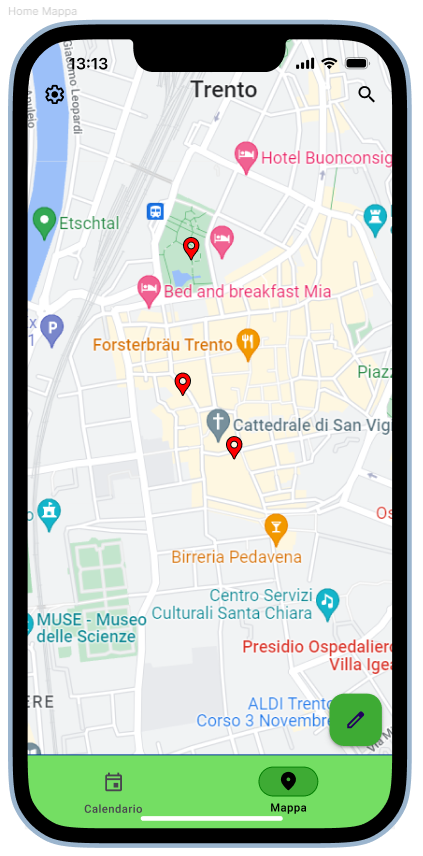
\includegraphics[scale=0.6]{Home_Mappa.png}
          \end{center}
    \item[] In questa schermata viene visualizzata la mappa con indicata la posizione degli eventi del giorno in base all'indirizzo scelto al momento della creazione.
    \item[] Cliccando su un "\faIcon{map-marker-alt}" si potranno visualizzare i dettagli dell'evento.
    \item[] Premendo l'icona "\faIcon{search}" si potrà ricercare un evento specifico
    \item[] Premendo l'icona "\faIcon{cog}" si potranno cambiare le impostazioni dell'account e di sistema
    \item[] Premendo l'icona "\faIcon{pencil-alt}" si potrà creare un nuovo evento \\ (visibile e utilizzabile solo se si dispone dell'autorizzazione necessaria: \textbf{UO}, \textbf{UA})
    \item[] È possibile passare dalla visualizzazione del calendario a quella della mappa tramite in basso presenti in entrambe le schermate.
\end{description}
\clearpage
\subsection{Pagina creazione evento}
\begin{description}
    \item[] Utenti utilizzatori: \textbf{UO}, \textbf{UA}
    \item[] Requisiti interessati: \hyperref[rf_5]{\textbf{RF5}}
    \item[] \begin{center}
              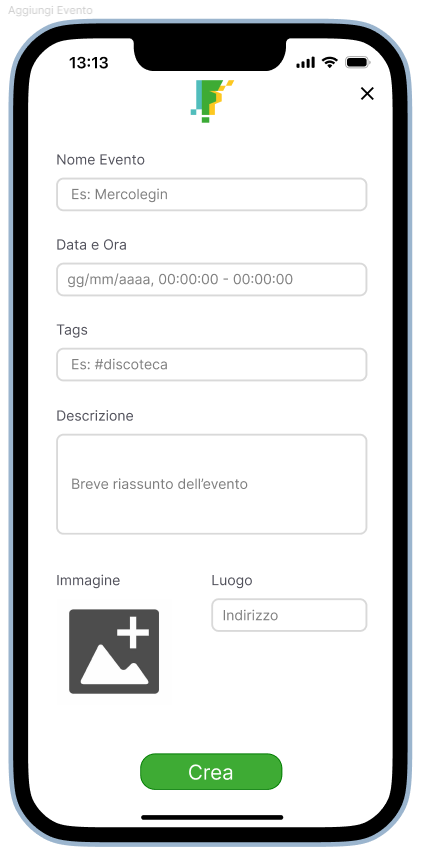
\includegraphics[scale=0.6]{Aggiungi_Evento.png}
          \end{center}
    \item[] In questa schermata è presente il form per la creazione di un nuovo evento
    \item[] L'utente deve inserire i dati richiesti (nome, data e ora, tags, descrizione, immagine e luogo) nei rispettivi campi presenti a schermo.
    \item[] È presente il tasto crea per confermare la creazione dell'evento o una croce in alto per annullare la compilazione.
\end{description}
\clearpage
\subsection{Pagina visualizza evento}
\begin{description}
    \item[] Utenti utilizzatori: \textbf{UNR}, \textbf{UR}, \textbf{UO}, \textbf{UA}
    \item[] Requisiti interessati: \hyperref[rf_3]{\textbf{RF3}}, \hyperref[rf_4]{\textbf{RF4}}
    \item[] \begin{center}
              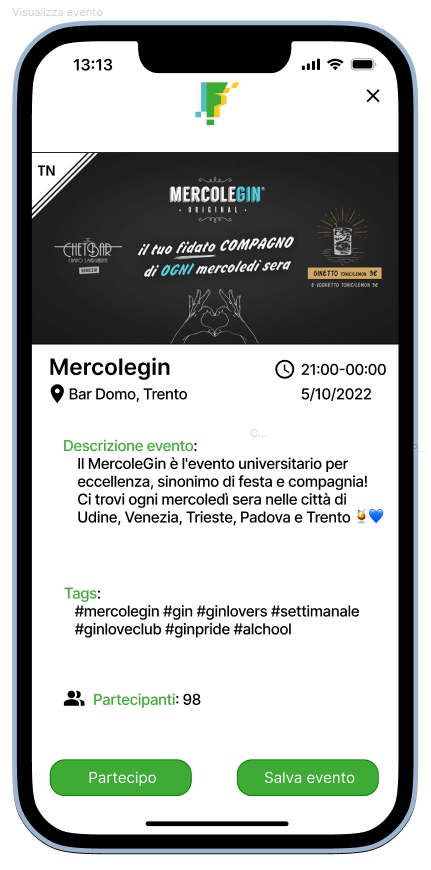
\includegraphics[scale=0.6]{Visualizza_Evento.png}
          \end{center}
    \item[] Vengono visualizzati a schermo i dettagli dell'evento selezionato: nome, immagine, descrizione, tag, data e ora, luogo, numero partecipanti.
    \item[] L'utente registrato ha accesso hai pulsanti "Partecipo" e "Salva Evento" che rispettivamente segnalano l'utente come partecipante o salvano l'evento nei preferiti dell'utente stesso.
    \item[] Se l'utente è l'organizzatore, o un admin, potrà inoltre visualizzare il tasto modifica.
\end{description}
\clearpage
\subsection{Pagina modifica evento}
\begin{description}
    \item[] Utenti utilizzatori: \textbf{UO}, \textbf{UA}
    \item[] Requisiti interessati: \hyperref[rf_6]{\textbf{RF6}}, \hyperref[rf_7]{\textbf{RF7}}
    \item[] La schermata è pressoché identica a quella della creazione evento, con unica differenza la rimozione del pulsante crea sostituito con "modifica" e "elimina".
\end{description}
\subsection{Pagina login}
\begin{description}
    \item[] Utenti utilizzatori: \textbf{UNR}
    \item[] Requisiti interessati: \hyperref[rf_8]{\textbf{RF8}}, \hyperref[rf_9]{\textbf{RF9}}
    \item[] Sono presenti 2 campi da compilare: e-mail, password.
    \item[] Se si ha dimenticato la password è presente un tasto per reimpostarla.
\end{description}
\clearpage
\subsection{Pagina impostazioni}
\begin{description}
    \item[] Utenti utilizzatori: \textbf{UNR}, \textbf{UR}, \textbf{UO}, \textbf{UA}
    \item[] Requisiti interessati: \hyperref[rf_10]{\textbf{RF10}}, \hyperref[rf_12]{\textbf{RF12}}, \hyperref[rf_13]{\textbf{RF13}}, \hyperref[rf_14]{\textbf{RF14}}, \hyperref[rf_15]{\textbf{RF15}}
    \item[] \begin{center}
              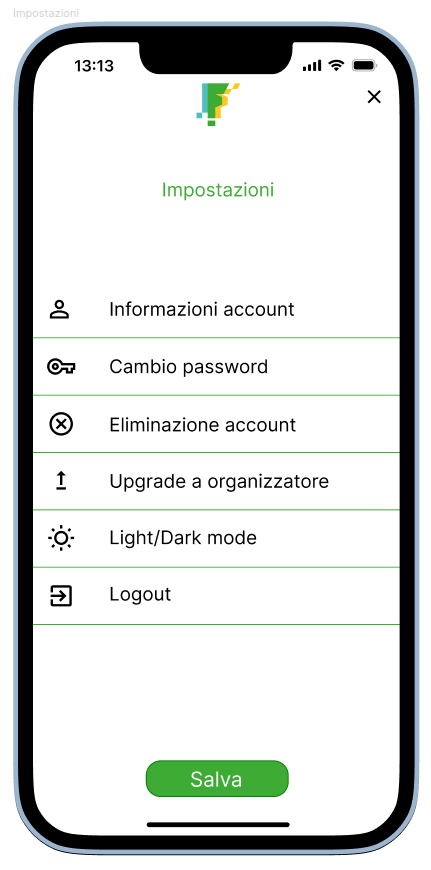
\includegraphics[scale=0.6]{Impostazioni.png}
          \end{center}
    \item[] Dalla pagina impostazioni è possibile accedere a diverse funzionalità:
          \begin{enumerate}
              \item creazione account \textbf{UNR}
              \item visualizzazione informazioni account \textbf{UR}, \textbf{UO}, \textbf{UA}
              \item modifica password \textbf{UR}, \textbf{UO}
              \item eliminazione account \textbf{UR}, \textbf{UO}
              \item richiesta upgrade ad account da organizzatore \textbf{UR}
              \item switch tema chiaro / scuro \textbf{UNR}, \textbf{UR}, \textbf{UO}, \textbf{UA}
              \item logout \textbf{UR}, \textbf{UO}, \textbf{UA}
          \end{enumerate}
    \item[] L'utente admin può inoltre elargire e revocare privilegi da organizzatore ad altri utenti inserendo la e-mail dell'interessato.
\end{description}
\subsection{Pagina creazione account}
\begin{description}
    \item[] Utenti utilizzatori: \textbf{UNR}
    \item[] Requisiti interessati: \hyperref[rf_10]{\textbf{RF10}}
    \item[] \begin{center}
              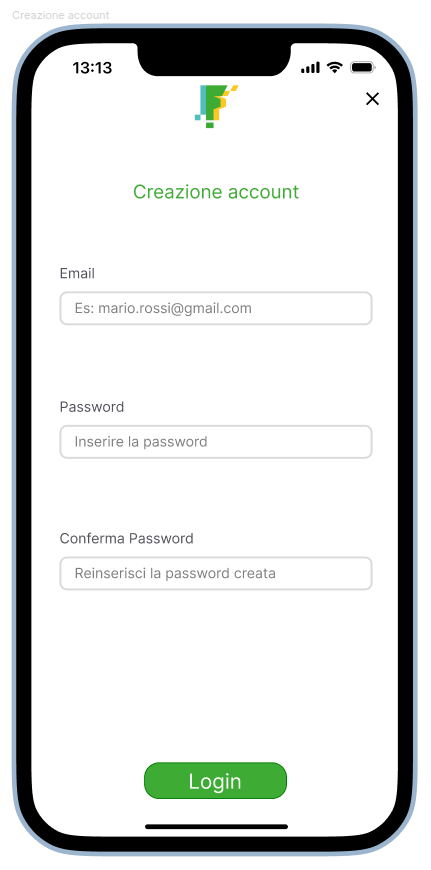
\includegraphics[scale=0.6]{Crea_Account.png}
          \end{center}
    \item[] L'utente deve compilare tre campi: e-mail, password, conferma password.
\end{description}
\clearpage
\section{Back-End}
Nel presente capitolo presentiamo i sistemi esterni con cui l’applicazione dovrà interagire per poter funzionare correttamente:
\begin{enumerate}
    \item \hyperref[leaflet]{Leaflet}
    \item \hyperref[TMS]{Transactional mail service}
    \item \hyperref[mongo]{Mongodb}
\end{enumerate}
\subsection{Leaflet \label{leaflet}}
\begin{description}
    \item[] Il sistema utilizza Leaflet per creare la mappa interattiva con indicatori customizzati per gli eventi giornalieri.
\end{description}
\subsection{Transactional Mail Service \label{TMS}}
\begin{description}
    \item[] Il sistema utilizza un Transactional Mail Service per ogni tipo di notifica automatica da inviare via mail agli utenti.
\end{description}
\subsection{Mongodb \label{mongo}}
\begin{description}
    \item[] Il sistema utilizza mongodb come database NOSQL in cui salvare dati relativi agli eventi e dati necessari all'autorizzazione dei diversi utenti.
\end{description}
\end{document}